\section{Simulação de Aplicações de Saúde Digital em WBANs}\label{castaliaapplayer}

%We have created an application for the Castalia Application Layer. This application is agent-initiated, that is, the agent takes the initiative to send readings to the manager. The agent is the first and the only one to send an \textit{Association request} to start sending measurements, as well as an \textit{Association release}, when there is no more measurements to be sent.
Este trabalho propõe o uso do padrão ISO/IEEE 11073 para simulação de aplicações de saúde digital em cenários de WBAN. Conforme o padrão, são propostos um componente gerente e outro agente na Camada de Aplicação do Simulador Castalia. 
O envio de dados pode ocorrer nos dois sentidos, do gerente para o agente ou do agente para o gerente. Porém, na implementação atual, o agente sempre inicia os envios de leituras para o gerente, simulando o envio de leituras de sensores ao nó concentrador da WBAN. O agente também é o primeiro e o único a enviar a mensagem de \textit{Association request} para solicitar uma associação ao gerente antes de iniciar o envio de leituras. Quando não há mais leituras para serem enviadas, o agente envia a mensagem \textit{Association release} para encerrar a associação. 

%The proposed application has five agent types, pulse oximeter, glucose meter, thermometer, blood pressure, and a basic ECG. The pulse oximeter transmits the pulse rate in beats per second and the Percentage of arterial hemoglobin oxygen saturation (SpO$_2$). The glucose meter sends the glucose level, that is, the concentration of glucose in the blood in milligrams per deciliter (mg\//dL). The thermometer measures temperature in Celsius (\textdegree C). The blood pressure sends a data compound of systolic, diastolic and the mean arterial pressure in millimeters of mercury (mmHg). The basic ECG sends eighty samples of the heart's electric potecial in millivolt (mV) per packet. Each mV sample has to be converted to scaled values before sent. 
%The lower and upper absolute values and the lower and upper scaled values are transmitted in the configuration phase. 
%All these agents samples are randomly produced, except the basic ECG that transmits real values obtained from a data base \cite{b2}.
A implementação atual oferece cinco dispositivos pessoais de saúde como agentes, um oxímetro de pulso, um medidor de glicose, um termômetro, um medidor de pressão e um eletrocardiograma (ECG de 3 derivações). O oxímetro transmite a frequência cardíaca em batimentos por minuto e a percentagem de saturação de oxigênio na hemoglobina arterial (SpO$_2$). O medidor de glicose transmite o nível de glicose, isto é, a concentração de açúcar no sangue em miligramas por decilitro (mg\//dL). O termômetro transmite a temperatura em Celsius (\textdegree C). O medidor de pressão envia uma mensagem composta por três medidas arteriais, sistólica, diastólica e a média arterial em milímetros de mercúrio (mmHg). O EGC envia oitenta amostras do potencial elétrico do coração em milivolts (mV) por pacote. 
%Cada amostra em $mV$ deve ser convertida para valores escalares antes de serem enviadas. 
%Os valores absolutos inferior e superior e os valores escalares inferior e superior são transmitidos na fase de configuração. 
Todos os dados dos agentes são produzidos de forma pseudo-aleatória, exceto o ECG que transmite valores reais obtidos a partir da base de dados \cite{b2}.

%The X73-PHD standard defines confirmed and unconfirmed events. The confirmed events expect a reception acknowledgment from the manager and the unconfirmed events do not. Control messages, like \textit{Association request} and \textit{Association release}, are always sent in confirmed mode, but measurements can be configured to use confirmed or unconfirmed mode. %The implemented parameter to set the desired mode is \textit{SN.node\[node number\].Application.confirmed\_event} which require a Boolean value.
A norma X73-PHD define eventos com confirmação e sem confirmação. Os eventos com confirmação esperam uma mensagem de reconhecimento do gerente enquanto os eventos sem confirmação não. Mensagens de controle como \textit{Association request} e \textit{Association release} são sempre eventos que esperam uma confirmação, porém o envio de leituras pode ser ou não confirmado.

%In this application, the user can also set some simulation's parameters like: the medical device type, thermometer, pulse oximeter, blood pressure and etc, the transmission rate in measurements per seconds, the mode of operation confirmed/unconfirmed, the retransmission of the packets rather than trying a new association and the maximum number of retransmission tries.
%Na aplicação proposta para o Castalia, os usuários também definir alguns parâmetros de simulação, que são: o tipo de dispositivo a ser simulado (termômetro, oxímetro de pulso, medidor de pressão sanguínea, medidor de glicose ou ECG), a taxa de transmissão de leituras por segundo, o modo de operação, com/sem confirmação ou optar em usar nossa proposta, o modo de retransmissão.  Neste último modo o número de tentativas de retransmissão e os \textit{timeouts} podem também ser alterados.

Se um agente usa o modo de comunicação confirmado e o ACK de uma leitura enviada ao gerente não chega, o padrão indica que o agente deve realizar uma nova associação com o gerente para transmitir novamente a leitura. Em um cenário de rede sem fio, a perda de quadros pode ocorrer com frequência, por isso, o modo de comunicação confirmado proposto no padrão pode levar a uma sobrecarga de pacotes de controle com necessidade de estabelecer uma nova associação toda vez que um ACK for perdido na WBAN.

Para contornar este problema, este artigo propõe um novo modo de comunicação chamado modo de retransmissão, como extensão ao padrão ISO/IEEE 11073. As próximas subseções detalham os três modos de operação e discutem como a proposta deste artigo pode melhorar o funcionamento de \textit{Personal Health Devices} em cenários WBANs.

\subsection{Eventos sem confirmação}\label{sec:UnconfirmedMeasurementEvent}

%Figure~\ref{fig:unconfirmedMode} shows a sequence diagram of the messaging process corresponding to an ordinary operation of an agent with standard configuration and with unconfirmed measurement events. The agent intends to associate with the manager for the first time, and sends an \textit{Association request}. When the manager receives the \textit{Association request}, it checks if the manager was previously associated. If it is the agent's first association, the manager sends a \textit{Get attributes} message along with the \textit{Association response}. So, the agent sends its configuration and starts to send the measurements to the manager. When there are no more readings to transmit, the agent sends an \textit{Association release} and the manager responds with an \textit{Association release response}.
A Figura \ref{fig:unconfirmedMode} mostra um diagrama de sequência do procedimento de troca de mensagens de uma operação normal de um agente com configuração padrão e usando eventos de envio de leituras sem confirmação. O agente pretende se associar com o gerente pela primeira vez e então envia um \textit{Association request}. Quando o gerente recebe o \textit{Association request}, ele verifica se já houve associações feitas previamente com esse agente. Se for a primeira associação, o gerente envia uma mensagem de \textit{Get attributes} juntamente com uma mensagem de \textit{Association response}. Logo após, o agente envia sua configuração e atributos para iniciar a transmissão de leituras. Quando todas as leituras tiverem sido enviadas, o agente envia uma mensagem de \textit{Association release} e o gerente responde com uma mensagem \textit{Association release response} para confirmar o término desta associação.

%\begin{figure}[htbp]
%\centerline{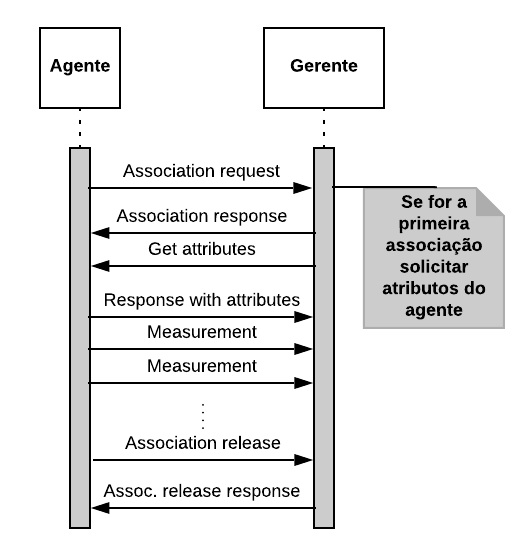
\includegraphics[scale=0.35]{figures/unconfirmed.png}}
%\caption{Sequence diagram of unconfirmed operation mode of an 11073 PHD application.}
%\label{fig:unconfirmedMode}
%\end{figure}

\begin{figure}[htbp]
\centering
\begin{minipage}{.5\textwidth}
\centering
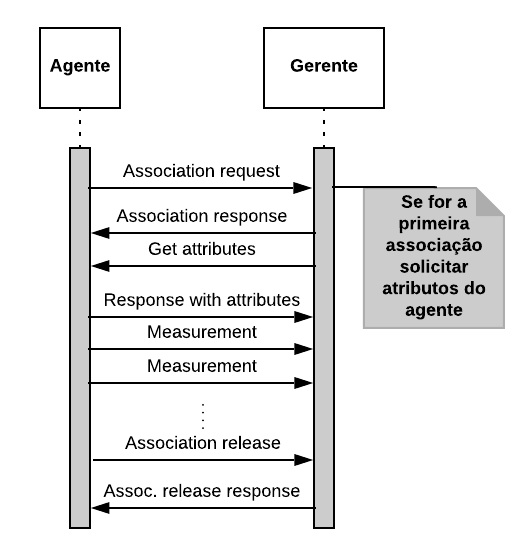
\includegraphics[width=.8\textwidth]{figures/unconfirmed.png}
\caption{Diagrama de sequência para o modo de operação sem confirmação de uma aplicação X73-PHD.}
\label{fig:unconfirmedMode}
\end{minipage}%
\begin{minipage}{.5\textwidth}
\centering
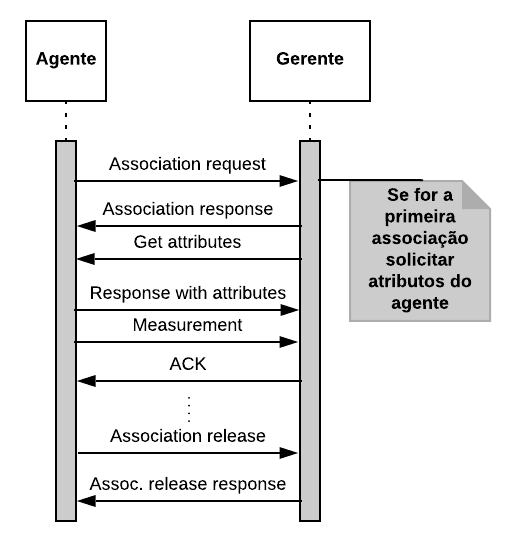
\includegraphics[width=.8\textwidth]{figures/confirmed.png}
\caption{Diagrama de sequência para o modo de operação com confirmação de uma aplicação X73-PHD.}
\label{fig:confirmedMode} 
\end{minipage}%
\end{figure}

\subsection{Eventos com confirmação}

%\begin{figure}[htbp]
%\centerline{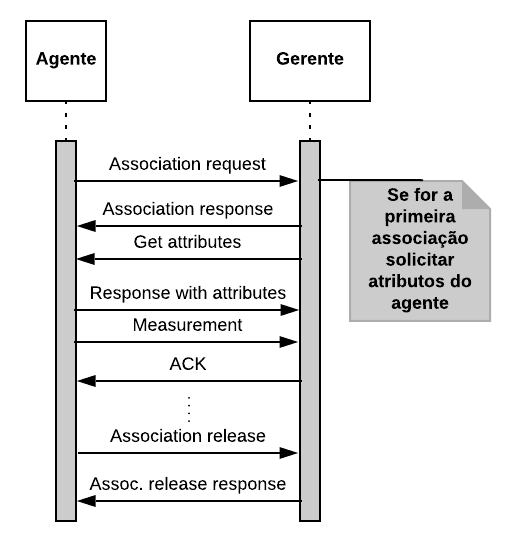
\includegraphics[scale=0.35]{figures/confirmed.png}}
%\caption{Sequence diagram of confirmed operation mode of an 11073 PHD application.}
%\label{fig:confirmedMode}
%\end{figure}

%\begin{figure}[htbp]
%\centering
%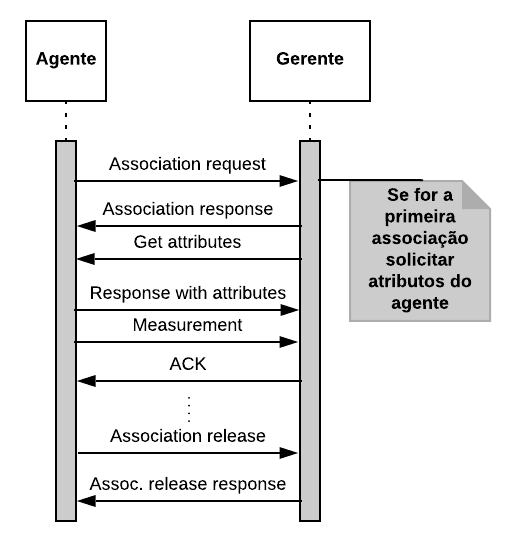
\includegraphics[width=.5\textwidth]{figures/confirmed.png}
%\caption{Diagrama de sequência para o modo de operação com confirmação de uma aplicação X73-PHD.}
%\label{fig:confirmedMode} 
%\end{figure}

%Figure~\ref{fig:confirmedMode} depicts a sequence diagram of the messaging procedure corresponding to an operation of an agent with standard configuration and with confirmed measurements events. The initial procedure is the same as explained in Section \ref{sec:UnconfirmedMeasurementEvent}, the difference is that the manager sends an acknowledgment for every measurement received. After sending a measurement data, the agent must wait three seconds for an ACK. If an ACK is not received in this period, the agent sends an \textit{Association abort} to the manager, and transits to the unassociated state. If the agent still has readings to send, a new association must be made. % VINICIUS - Reescreve isso aí, pq não deu pra entender - This and others errors conditions is explained in \cite{b1}.
A Figura \ref{fig:confirmedMode} descreve o diagrama de sequência da operação de um agente com configuração padrão usando eventos de envio de leitura com confirmação. O processo inicial é idêntico ao explicado na Seção \ref{sec:UnconfirmedMeasurementEvent}. A diferença é que para cada leitura que o agente envia, o gerente confirma com uma mensagem ACK. Após enviar uma leitura, o agente espera a confirmação por três segundos, se nada chegar durante esse período, o agente envia uma mensagem de interrupção, \textit{Association abort}, e transita para o estado de máquina não associado. Se ainda existirem leituras para serem enviadas, o agente deve tentar uma nova associação.

\subsection{Proposta de Modo de Retransmissão}

%The X73-PHD standard assumes that there will be a reliable transport layer on real devices. In the Castalia simulator, as in usual wireless sensor networks, a transport layer is not used. So we propose a stop-and-wait system as a sub-application-layer to retransmit agent packets whose ACK have not been received.
O padrão X73-PHD assume que, em dispositivos reais, haverá um camada de transporte confiável disponível para comunicação. Em uma WBAN, pode não haver camada de transporte confiável disponível, já que os sensores têm poucos recursos de memória, processamento e bateria. Desta forma, este artigo propõe um novo modo de comunicação, baseado em \textit{stop-and-wait}, para realizar retransmissões de pacotes perdidos ou não confirmados pelo gerente.

%To avoid many associations right after a non-received ACK we implemented a stop-and-wait retransmission system in the application layer. 
%It reduces the unnecessary exchange of several control packets made in association procedures. Rather than making a new association when an ACK is lost, we just retransmit the packet $n$ times or until an ACK is received.
%The user can define whether to retransmit and how many retransmission attempts wish.
%The user may define a number ($n$) of retransmissions, and the agent will retransmit that message up to $n$ times until a corresponding ACK is received. If the manager receives a duplicated message, it will retransmit immediately another ACK to the agent.
Isso reduz a troca desnecessária de vários pacotes de controle no processo de associação. Ao invés de fazer uma nova associação quando um ACK não é recebido, retransmite-se o pacote até que um ACK seja recebido. O usuário define o número $n$ de retransmissões, e, então, aquela leitura será retransmitida até $n$ vezes ou até que um ACK seja recebido. Se o gerente receber uma mensagem duplicada, ele retransmitirá imediatamente o ACK que não foi recebido pelo agente, ou seja, o último ACK enviado.

Na fase de associação, a implementação reduz o \textit{timeout} de $10$ para $0.4$ segundos. Após a associação, o dispositivo usando o \textit{o Modo de Retransmissão}, envia sua primeira leitura, aguarda o período de \textit{timeOutToRetransmitPacket} conforme definido pelo usuário no arquivo de configuração da simulação. Se nenhuma resposta for recebida, o pacote é retransmitido no máximo \textit{maxNumOfRetransmition} vezes, conforme definido também pelo usuário, ou até que uma mensagem de reconhecimento do gerente seja recebida. Se todas as tentativas definidas em \textit{maxNumOfRetransmition} forem utilizadas, então uma nova associação é feita com o gerente e a variável \textit{maxNumOfRetransmition} é redefinida para $0$. Esse processo continua até o agente realizar $3$ associações, conforme definido na norma X73-PHD. Na quarta tentativa, o agente envia uma mensagem de \textit{Association abort} e volta para estado de máquina \textit{não associado}. 

%In Section \ref{results}, we evaluate this solution's efficiency in reducing control packets exchange in a WBAN scenario. Note that this is a new proposal, not present in the X73-PHD standard. 
%The parameters implemented for retransmission are \textit{SN.node[nodeNumber].Application.retransmissionPacket} which require a boolean value and \textit{SN.node[nodeNumber].Application.maxNumOfRetransmition} that accepts an integer number.
Na Seção \ref{results}, é avaliada a eficiência desta proposta usando como métrica a redução no envio de pacotes de controle, o número de novas associações feitas por cada dispositivo, a quantidade de pacotes retransmitidos e a número de leituras transmitidas com sucesso para o gerente. Vale ressaltar que esta é uma nova proposta e não está presente na norma X73-PHD.

A implementação no simulador Castalia foi realizada utilizando a biblioteca Antidote \cite{b20} como base. Ao usar a nova camada de aplicação disponível, os usuários também podem definir alguns parâmetros de simulação, que são: o tipo de dispositivo a ser simulado (termômetro, oxímetro de pulso, medidor de pressão sanguínea, medidor de glicose ou ECG), a taxa de transmissão de leituras por segundo, o modo de operação, com/sem confirmação ou optar em usar a proposta deste artigo, o modo de retransmissão.  Neste último modo, o número de tentativas de retransmissão e os \textit{timeouts} também podem ser configurados.
